\subsection{Método Robertson} \label{metodoRobertson}

O método proposto por Robertson \etal~\cite{robertson} aborda a geração de imagens HDR de maneira similar ao método proposto por Mann e Picard (Subseção \ref{metodoMann}). Esse método utiliza a derivada da função resposta em um eixo logarítmico como peso e assume que as imagens são estáticas entre si, variando apenas o tempo de exposição. As principais diferenças entre os dois métodos são a postura adotada em relação ao tratamento do ruído e a forma como a função resposta da câmera é inferida. Neste caso a função resposta é inferida por meio de um método iterativo que supõe uma função inicial padrão e então, com uso da relaxação de Gauss-Seidel, aproxima a função resposta de forma a obter um erro abaixo de um limiar estabelecido.

\subsubsection{Geração da Imagem HDR} \label{metodoRobertsonGeracao}

Ao tentar extrair o valor de irradiação de luz ao qual um pixel é mapeado, aplica-se a inversa da função resposta. No entanto, no momento de registro da imagem, vários fatores influenciam para que o valor registrado seja ligeiramente diferente do valor ideal. Isso se dá por conta da presença do ruído no ambiente, que pode ser advindo de fontes diferentes, como corrente de escuro, conversão de analógico para digital entre outros. Assim, a equação da inversa da função resposta da câmera pode ser descrita da seguinte maneira:

\begin{align} \label{eqRobertsonIFR}
	f_{(p_{ij})}^{-1} = I_{p_{ij}} = xt_{i} + N_{ij}
\end{align}
Onde
\begin{itemize}
\item $N_{ij}$ encapsula os ruídos tiveram influência na captura do pixel.
\item $x$ é o valor de irradiação de luz real que deseja-se encontrar.
\item $t_{i}$ é o tempo de exposição ao qual o sensor da câmera foi submetido para captura do pixel.
\item $p_{ij}$ é o valor do pixel $j$ da imagem com exposição $t_{i}$.
\end{itemize}

Como o ruído é uma caracteristica singular para cada ambiente/câmera utilizada, modelar o problema de forma a caracterizar cada ruído é uma tarefa bastante complexa. Sendo assim, este método trata o ruído sob o ponto de vista de uma distribuição gaussiana com média zero para simplificar a modelagem.

Utilizando-se de operações algébricas para calcular o erro de um valor de iluminação inferido em relação ao valor real, obtém-se a seguinte equação:

\begin{align} \label{eqRobertsonErr}
	O(x) = \sum\limits_{i,j}{w_{ij}(I_{p_{ij}} - x_{ij}t_{i})^2}
\end{align}

Essa equação representa o erro quadrático entre o valor inferido e o valor obtido pela inversa. Fazendo o gradiente de $O(x)$ tender a zero, os autores do método chegaram à seguinte equação para inferência do valor de irradiação de luz:

\begin{align} \label{eqRobertsonGeracao}
	x^{*}_j = \frac{\sum{_i w_{ij}t_{i}I_{p_{ij}}}}{\sum{_i w_{ij}t_{ij}^{2}}}
\end{align}
Onde
\begin{itemize}
\item $x^{*}_j$ é o valor de irradiação de luz inferido.
\item O peso $w_{ij}$ é obtido pela derivada da função resposta em relação um eixo logarítmico. 
\end{itemize}

O conjunto de valores $x^{*}_j$, que são gerados a partir da convolução das imagens de entrada, formam a imagem HDR final.

\subsubsection{Algoritmo para Inferir a Função Resposta} \label{metodoRobertsonAlg}

Na maioria dos casos, não se sabe a função resposta de uma câmera e por isso ela deve ser estimada \cite{robertson}. Para a estimativa da função resposta é necessária a minimização da função do erro quadrático, dada pela seguinte equação:

\begin{align} \label{eqRobertsonErr2}
	O(I,x) = \sum\limits_{i,j}{w_{ij}(I_{p_{ij}} - x_{ij}t_{i})^2}
\end{align}

Essa equação é parecida com a Equação \ref{eqRobertsonErr}, porém com uma variável $I$ de entrada que também será inferida. Como não se sabe o valor de irradiação $x_{ij}$ nem a função resposta para calcular o valor de $I_{p_{ij}}$, utiliza-se o método de relaxação de Gauss-Seidel para inferir ambas as variáveis simultaneamente. Também é necessário estabelecer uma função para mapear os pesos uma vez que, como não se sabe a função resposta da câmera, não há como obter a sua derivada. Os autores propõem a seguinte função para definir os pesos \cite{robertson2}:

\begin{align} \label{eqRobertsonErr3}
	w_{ij} = e^{-4\frac{(p_{ij}-127.5)^2}{127.5^2}}
\end{align}

O método de inferência da fução resposta possui um passo inicial e um conjunto de passos iterativos, descritos a seguir.

\begin{itemize}
\item Passo inicial:

Estabelece-se a função resposta inicial como sendo uma função linear com o valor $I_{128}^{*(0)} = 1.0$, e o valor de $x^{*(0)}$ é obtido aplicando a equação \ref{eqRobertsonGeracao}.

\item Passos iterativos:

Para cada iteração $l$ são feitos os seguintes passos:
\subitem \textbf{1.} Considerando $E_m$ o conjunto de pixels que possuem o valor igual a $m$, faz-se o relaxamento de $I^{*(l)}$ aplicando a seguinte Equação para inferi-lo:
\begin{align} \label{eqRobertsonIteracaoFR}
	I^{*(l)}_m = \frac{\sum\limits_{(i,j) \in E_m}{w_{ij}t_{i}x_{j}^{*(l-1)}}}{\sum\limits_{(i,j) \in E_m}{w_{ij}}}
\end{align}
\subitem \textbf{2.} Normaliza-se $I_{p_{ij}}$ de forma que $I_{128}$ seja uma unidade.
\subitem \textbf{3.} É feita a relaxação de $x^{*(l)}$ com base na seguinte equação:
\begin{align} \label{eqRobertsonIteracaoHDR}
	x^{*(l)}_j = \frac{\sum{_i w_{ij}t_{i}I^{*(l)}_{p_{ij}}}}{\sum{_i w_{ij}t_{i}^2}}
\end{align}
\end{itemize}

Dessa forma, a função resposta e a imagem HDR vão sendo inferidas simultaneamente, e quando as modificações feitas no passo iterativo da Equação \ref{eqRobertsonIteracaoFR} forem menores que um limiar predefinido o passo iterativo é terminado.

Ao final do método, possui-se um conjunto de valores $\{I_{p_{ij}}\}$ que representam informações da função resposta da câmera. Como este conjunto é discreto, há a necessidade de efetuar uma interpolação utilizando a técnica da Spline cúbica (vide Seção \ref{conceitoSpline}) para obtenção da função resposta final como ilustrado na Figura \ref{figRobertsonPontos}. 

\begin{figure}[H]
  \centering
  \subfloat[Ilustração dos pontos utilizados na interpolação.]
  {
    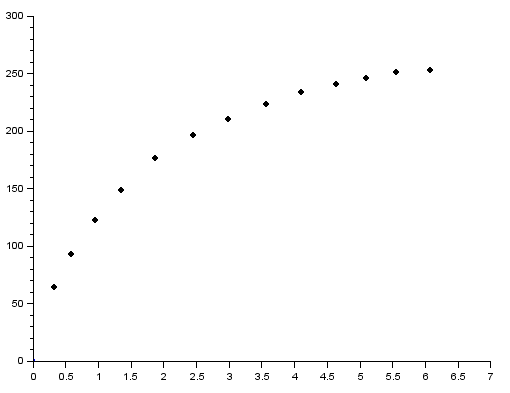
\includegraphics[height=6cm]{Robertson/Pontos}
    \label{figRobertsonPontosA}
  }
  \quad %espaco separador
  \subfloat[Função resposta obtida com a interpolação.]
  {
    \includegraphics[height=6cm]{Robertson/fr-linear-azul}
    \label{figRobertsonPontosB}
  }
  \caption{Interpolação da função resposta do canal azul da câmera, utilizando o método da Spline cúbica.}
  \label{figRobertsonPontos}
\end{figure}

\subsubsection{Resultados e Discussões} \label{metodoRobertsonResultado}

O método em questão foi implementado na linguagem de programação C++, assim como o método de interpolação por spline cúbica. Os resultados são mostrados nas Figuras \ref{figRobertsonDidatica}, \ref{figRobertsonPorquinho} e \ref{figRobertsonOlhinhos}.

\begin{figure}[H]
  \centering
  \subfloat[Imagem visualizada com ganho de -11,0EV.]
  {
    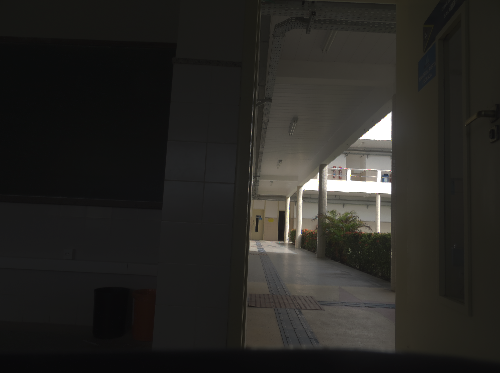
\includegraphics[height=6cm]{Robertson/robertsonSala-11,0EV}
    \label{figRobertsonDidaticaA}
  }
  \quad %espaco separador
  \subfloat[Imagem visualizada com de ganho -4,3EV.]
  {
    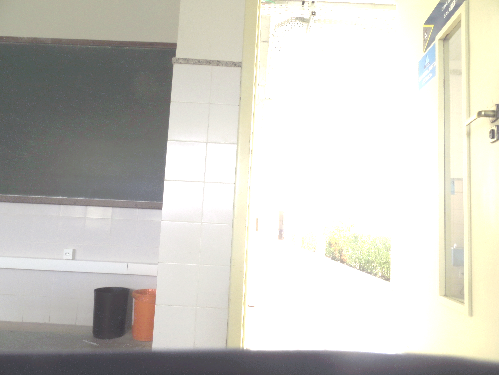
\includegraphics[height=6cm]{Robertson/robertsonSala-4,3EV}
    \label{figRobertsonDidaticaB}
  }
  \caption{Imagem HDR gerada utilizando o método de Robertson~\etal~\protect\cite{robertson}.}
  \label{figRobertsonDidatica}
\end{figure}

\begin{figure}[H]
  \centering
  \subfloat[Imagem visualizada com ganho de -4,3EV.]
  {
    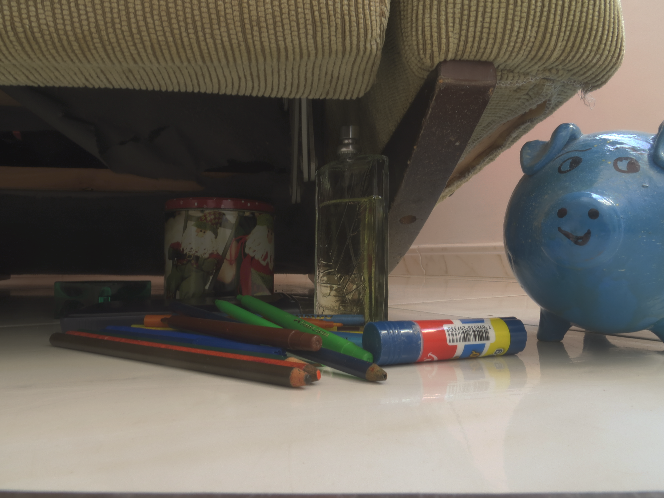
\includegraphics[height=6cm]{Robertson/robertsonOtima-4,3EV}
    \label{figRobertsonPorquinhoA}
  }
  \quad %espaco separador
  \subfloat[Imagem visualizada com ganho de -2,0EV.]
  {
    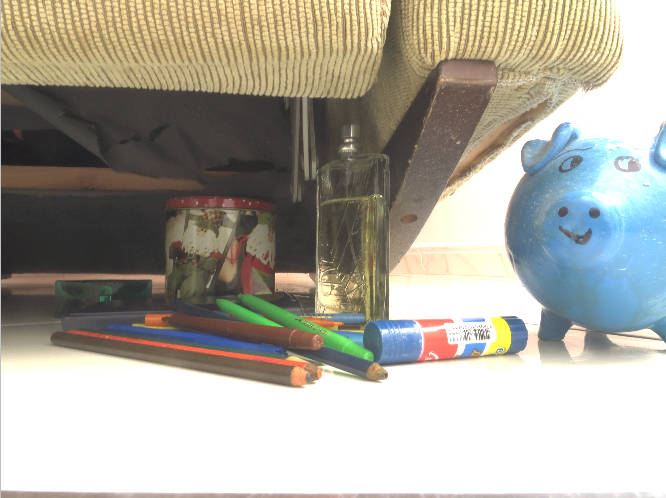
\includegraphics[height=6cm]{Robertson/robertsonOtima-2,0EV}
    \label{figRobertsonPorquinhoB}
  }
  \quad %espaco separador
  \subfloat[Imagem visualizada com ganho de 0EV.]
  {
    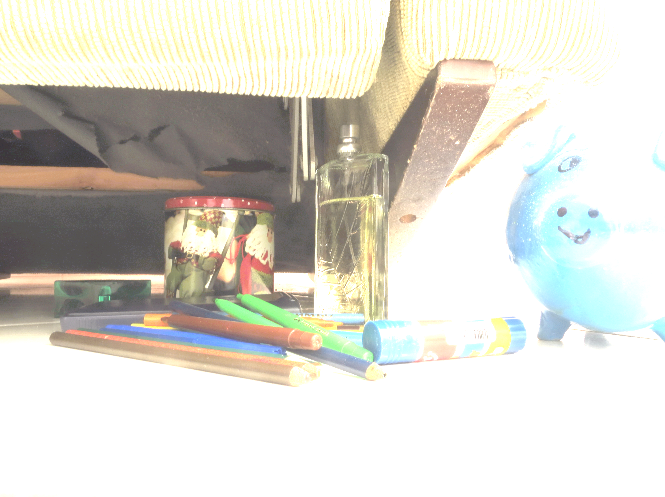
\includegraphics[height=6cm]{Robertson/robertsonOtima0,0EV}
    \label{figRobertsonPorquinhoC}
  }
  \caption{Imagem HDR gerada utilizando o método de Robertson~\etal~\protect\cite{robertson}.}
  \label{figRobertsonPorquinho}
\end{figure}


\begin{figure}[H]
  \centering
  \subfloat[Imagem visualizada com ganho de -4,3EV.]
  {
    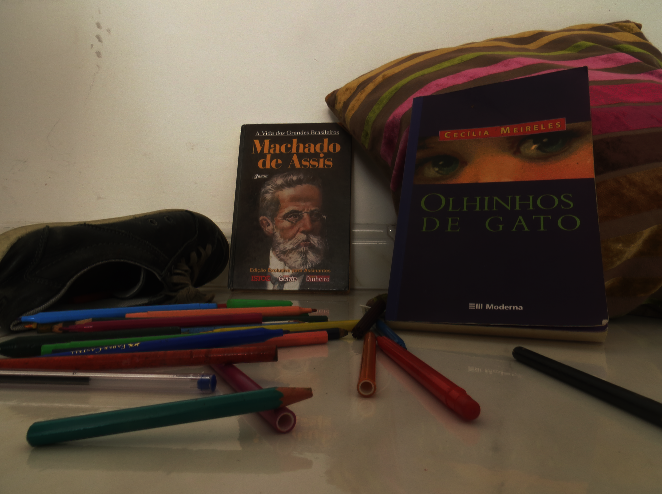
\includegraphics[height=6cm]{Robertson/robertsonOlhinhos-4,3EV}
    \label{figRobertsonOlhinhosA}
  }
  \quad %espaco separador
  \subfloat[Imagem visualizada com ganho de -2,7EV.]
  {
    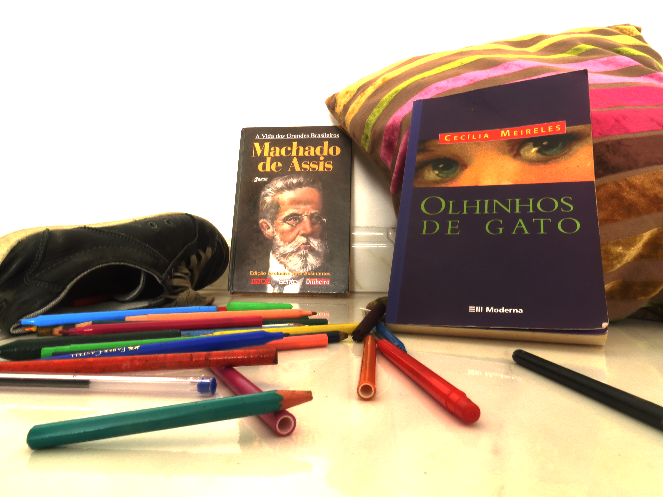
\includegraphics[height=6cm]{Robertson/robertsonOlhinhos-2,7EV}
    \label{figRobertsonOlhinhosB}
  }
  \quad %espaco separador
  \subfloat[Imagem visualizada com ganho de -0,4EV.]
  {
    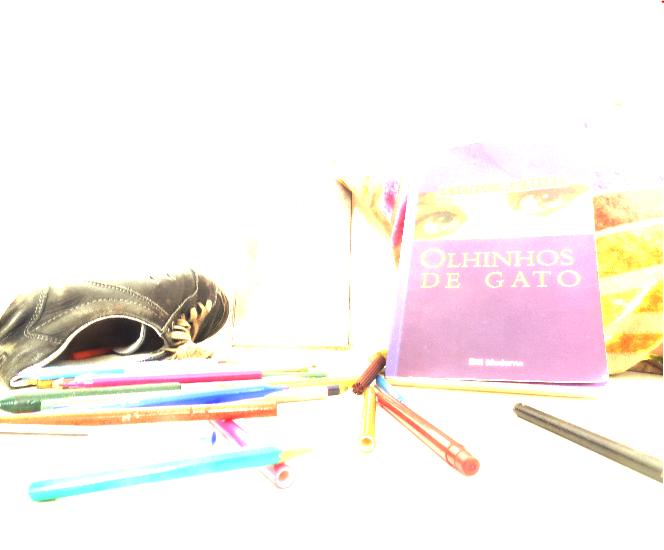
\includegraphics[height=6cm]{Robertson/robertsonOlhinhos-0,4EV}
    \label{figRobertsonOlhinhosC}
  }
  \caption{Imagem HDR gerada utilizando o método de Robertson~\etal~\protect\cite{robertson}.}
  \label{figRobertsonOlhinhos}
\end{figure}


\begin{figure}[H]
  \centering
  \subfloat[Imagem HDR gerada]
  {
    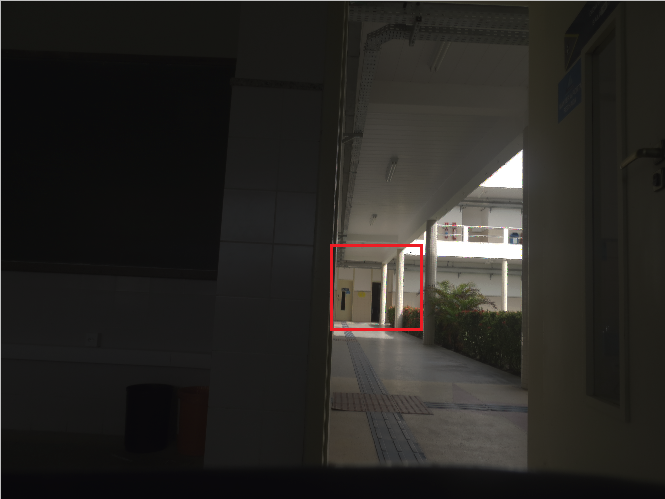
\includegraphics[height=6cm]{Robertson/Sala}
    \label{figRobertsonSalaA}
  }
  \quad %espaco separador
  \subfloat[A aproximação mostrou a presença de ruído na imagem]
  {
    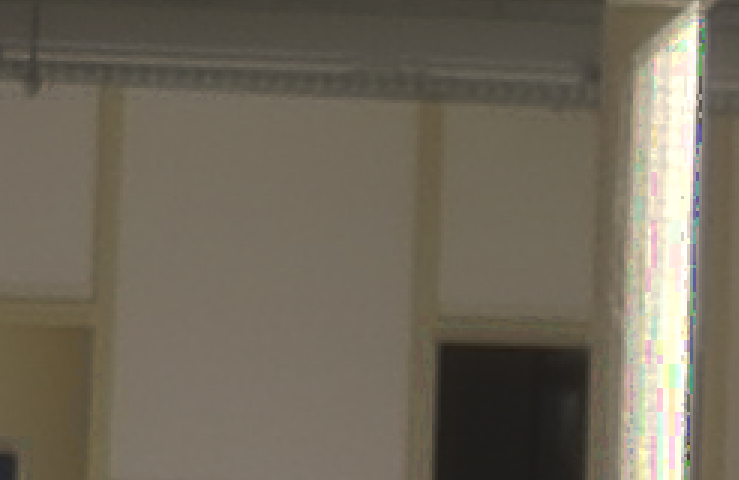
\includegraphics[height=6cm]{Robertson/Ruido}
    \label{figRobertsonSalaB}
  }
  \caption{Imagem HDR gerada utilizando o método de Robertson~\etal~\protect\cite{robertson}, que apresentou ruído em partes com muita irradiação de luz.}
  \label{figRobertsonSala}
\end{figure}

Notou-se que áreas com exposição muito elevada apresentaram ruído mais perceptível, como mostrado na Figura \ref{figRobertsonSalaB}. E a Figura \ref{figRobertsonFR} mostra as funções resposta dos diferentes canais, obtidas utilizando o método proposto.

\begin{figure}[H]
  \centering
  \subfloat[Eixo linear]
  {
    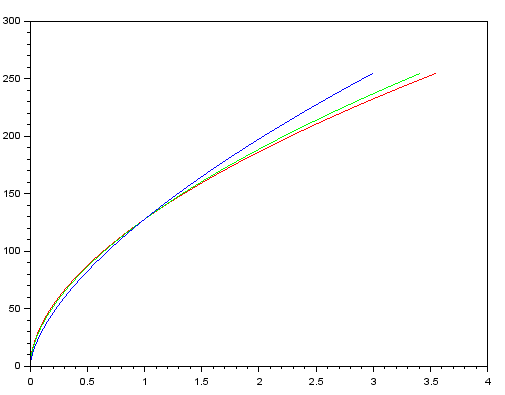
\includegraphics[height=6cm]{Robertson/fr-linear-total}
    \label{figRobertsonFRA}
  }
  \quad %espaco separador
  \subfloat[Eixo logarítmico]
  {
    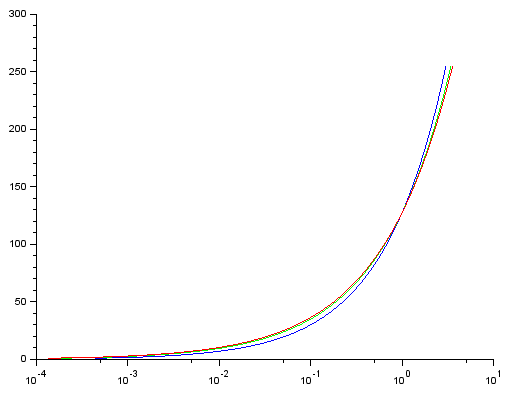
\includegraphics[height=6cm]{Robertson/fr-log-total}
    \label{figRobertsonFRB}
  }
  \caption{Funções resposta da câmera relativas aos diferentes canais de cores.}
  \label{figRobertsonFR}
\end{figure}

